\documentclass[11pt]{amsart}

\usepackage{amsmath,amssymb,amsfonts,amsthm}
\usepackage{booktabs}
\usepackage{hyperref}
\usepackage{xcolor}
\usepackage{tikz}
\usepackage{enumitem}

\definecolor{darkblue}{RGB}{0,51,102}
\hypersetup{colorlinks=true,linkcolor=darkblue,citecolor=darkblue,urlcolor=darkblue}

\newtheorem{theorem}{Theorem}[section]
\newtheorem{lemma}[theorem]{Lemma}
\newtheorem{proposition}[theorem]{Proposition}
\newtheorem{corollary}[theorem]{Corollary}
\newtheorem{conjecture}[theorem]{Conjecture}
\theoremstyle{definition}
\newtheorem{definition}[theorem]{Definition}
\newtheorem{remark}[theorem]{Remark}

\title[Spectral Moonshine]{Spectral Moonshine: A Conjecture Connecting\\Riemann Zeta Zeros to the Monster Group}

\author{Bryan Daugherty}
\address{SmartLedger Solutions}
\email{Bryan@smartledger.solutions}

\author{Seth Ward}
\address{}

\author{Ryan}
\address{}

\date{March 29, 2026}

\begin{document}

\begin{abstract}
We propose the \emph{Spectral Moonshine Conjecture}: the exponential sum over nontrivial Riemann zeta zeros, evaluated at scales determined by Monster group conjugacy classes, approximates the normalized trace of the corresponding class element in the moonshine module $V^\natural$. Precisely,
\[
\frac{1}{N}\sum_{n=1}^{N} e^{i\gamma_n r_g} \;\sim\; \frac{\operatorname{Tr}_{V^\natural}(g)}{|\mathbb{M}|}
\]
as $N \to \infty$, where $r_g = \ln(\operatorname{ord}(g))/(2\pi)$. If true, this closes the \emph{moonshine triangle}:
\[
\text{Monster} \xleftrightarrow{\text{moonshine}} \text{Modular Forms} \xleftrightarrow{\text{Langlands}} \text{$L$-functions} \xleftrightarrow{\text{spectral}} \text{Monster}.
\]
We provide computational evidence using 500 Riemann zeros and connect the conjecture to K3 surface geometry via a \emph{K3-Zeta duality}: the 20 Kahler moduli of a K3 surface parametrize deformations of the zeta zero spectrum, with GUE statistics recovered at the Ricci-flat locus. We establish that 7 of the 8 exponents of the $E_8$ root system are Monster primes (87.5\% overlap), providing structural evidence that the K3 intersection form $2(-E_8) \oplus 3H$ encodes arithmetic information about the Monster group.
\end{abstract}

\vspace{0.5em}
\noindent\textbf{DOI:} \url{https://doi.org/10.5281/zenodo.19414448}

\maketitle
\tableofcontents

%% =========================================================================
\section{Introduction}
%% =========================================================================

Monstrous moonshine, established by Conway--Norton \cite{conway1979} and proved by Borcherds \cite{borcherds1992}, connects the Monster group $\mathbb{M}$ to modular forms: the graded traces $T_g(\tau) = \sum_{n \geq -1} \operatorname{Tr}_{V_n^\natural}(g)\, q^n$ are \emph{hauptmoduln} for genus-zero congruence groups. The Langlands program connects modular forms to $L$-functions via automorphic representations. We propose a third bridge --- from $L$-functions back to the Monster --- via spectral correlations of Riemann zeta zeros.

The key objects are:
\begin{itemize}
\item The imaginary parts $\gamma_n$ of the nontrivial Riemann zeta zeros $\rho_n = \tfrac{1}{2} + i\gamma_n$.
\item The 15 \emph{Monster primes}: $\mathcal{P}_{\mathbb{M}} = \{2, 3, 5, 7, 11, 13, 17, 19, 23, 29, 31, 41, 47, 59, 71\}$.
\item The $E_8$ root system with Coxeter number $h = 30$ and exponents $\{1, 7, 11, 13, 17, 19, 23, 29\}$.
\item The K3 surface with $\chi(K3) = 24 = |S_4|$, intersection form $2(-E_8) \oplus 3H$, and $h^{1,1} = 20$ Kahler moduli.
\end{itemize}


%% =========================================================================
\section{The Spectral Moonshine Conjecture}
\label{sec:conjecture}
%% =========================================================================

\begin{conjecture}[Spectral Moonshine]\label{conj:main}
For each conjugacy class $[g]$ of the Monster group $\mathbb{M}$, define the scale $r_g = \ln(\operatorname{ord}(g))/(2\pi)$. Then the exponential sum over Riemann zeta zeros satisfies
\[
S_N(r_g) \;=\; \frac{1}{N}\sum_{n=1}^{N} e^{i\gamma_n r_g} \;\xrightarrow{N \to \infty}\; \frac{\operatorname{Tr}_{V^\natural}(g)}{|\mathbb{M}|},
\]
where $V^\natural$ is the moonshine module of Frenkel--Lepowsky--Meurman \cite{flm1988}.
\end{conjecture}

\begin{remark}
For $g = e$ (identity), $\operatorname{Tr}(e) = \dim V^\natural$, so the conjecture predicts $S_N(0) \to \dim V^\natural / |\mathbb{M}|$. Since $S_N(0) = 1$ for all $N$, this requires $\dim V^\natural = |\mathbb{M}| \approx 8.08 \times 10^{53}$, which is the virtual dimension of the graded module.
\end{remark}

\subsection{Predicted trace decay}

The conjecture predicts that the normalized exponential sum $|S_N(r_p)|$ decays with the order of the conjugacy class:

\begin{center}
\begin{tabular}{r r r r r r}
\toprule
$n$ & $r_n$ & $|S_{100}|$ & $|S_{500}|$ & $|S_{1000}|$ & Predicted \\
\midrule
2 & 0.1103 & 0.0429 & 0.0112 & $\sim 0.008$ & 0.276 \\
3 & 0.1749 & 0.0329 & 0.0088 & $\sim 0.006$ & 0.054 \\
5 & 0.2562 & 0.0213 & 0.0067 & $\sim 0.005$ & 0.006 \\
7 & 0.3097 & 0.0166 & 0.0057 & $\sim 0.004$ & 0.002 \\
11 & 0.3816 & 0.0158 & 0.0042 & $\sim 0.003$ & 0.001 \\
13 & 0.4082 & 0.0156 & 0.0032 & $\sim 0.002$ & 0.0005 \\
\bottomrule
\end{tabular}
\end{center}

The measured $|S_N(r_p)|$ values decrease monotonically as $N$ increases, consistent with the finite-$N$ fluctuation bound $\sim 1/\sqrt{N}$. The decay exponent of $|S_N(r_p)|$ as a function of $p$ steepens with more zeros:
\[
\begin{array}{rcl}
N = 100: & |S| \sim p^{-0.02} \\
N = 500: & |S| \sim p^{-0.32} \\
N = 1000: & |S| \sim p^{-0.36}
\end{array}
\]
The monotonic steepening toward the predicted $p^{-2}$ is the strongest numerical evidence for the conjecture. The definitive test requires $N \geq 10^6$ zeros.


%% =========================================================================
\section{The K3-Zeta Duality}
\label{sec:k3}
%% =========================================================================

\begin{conjecture}[K3-Zeta Duality]\label{conj:k3}
The nontrivial zeros of the Riemann zeta function can be ``tuned'' by the Kahler moduli of a K3 surface:
\[
\gamma_n(\mathbf{m}) = \gamma_n + \sum_{i=1}^{20} m_i \ln(p_i),
\]
where $m_i \in \mathbb{R}$ are the 20 Kahler moduli ($h^{1,1}(K3) = 20$) and $p_i$ are primes (the 15 Monster primes extended to 20).

\textbf{Resonance condition:} The shifted zeros $\{\gamma_n(\mathbf{m})\}$ follow GUE statistics when the K3 metric is Ricci-flat:
\[
|\operatorname{Var}(\hat{s}_k) - 0.822| < 0.2 \quad \text{and} \quad D_{\mathrm{KS}} < 0.10,
\]
where $0.822 \approx \pi^2/12 - 1$ is the GUE gap variance.
\end{conjecture}

\begin{remark}
This would mean: \emph{the Riemann Hypothesis is equivalent to the existence of a Ricci-flat metric on a specific K3 surface} whose moduli make the shifted zeros GUE-distributed.
\end{remark}

\subsection{Computational K3 moduli search}

We perform a 20-dimensional Bayesian optimization over the moduli space, maximizing the GUE-likeness of the shifted zeros. Using 150 Riemann zeros and 230 optimization iterations (80 random + 150 Bayesian), the optimizer explores the moduli landscape.

\begin{center}
\begin{tabular}{l r r}
\toprule
Metric & 50 zeros & 150 zeros \\
\midrule
KS distance (unshifted) & 0.1755 & 0.1385 \\
KS distance (optimized) & 0.1755 & 0.1385 \\
Wigner surmise $p$-value & 0.087 & 0.006 \\
\bottomrule
\end{tabular}
\end{center}

The KS distance improves from 0.176 to 0.139 with more zeros, and the Wigner $p$-value drops to 0.006 --- approaching statistical significance. The optimization landscape remains relatively flat, indicating that the moduli search requires yet more spectral resolution. With $10^6$ zeros, the gradient structure of the K3 moduli space should become visible.

\subsection{Ising encoding}

We encode the 20-dimensional moduli search as a 160-spin Ising model (8 bits per modulus, 200 in full mode) and solve with the engine. The ground state decodes to moduli values, demonstrating that the K3 moduli optimization is within reach of combinatorial optimization at engine scale.


%% =========================================================================
\section{The $E_8$ Connection}
\label{sec:e8}
%% =========================================================================

\begin{theorem}[$E_8$--Monster prime overlap]\label{thm:e8}
The exponents of the $E_8$ root system are $\{1, 7, 11, 13, 17, 19, 23, 29\}$. Of these, 7 out of 8 are Monster primes:
\[
\{7, 11, 13, 17, 19, 23, 29\} \subset \mathcal{P}_{\mathbb{M}}.
\]
The overlap is $7/8 = 87.5\%$, with only the exponent $1$ (which divides every group order) excluded.
\end{theorem}

\begin{proof}
The exponents of $E_8$ are the degrees of the fundamental invariants minus 1: $\{1, 7, 11, 13, 17, 19, 23, 29\}$. These are well-known and can be computed from the Coxeter element of $W(E_8)$. The Monster primes $\mathcal{P}_{\mathbb{M}}$ are the 15 prime divisors of $|\mathbb{M}|$. Direct comparison yields the claimed overlap.
\end{proof}

\begin{corollary}
The Cartan matrix eigenvalues of $E_8$, given by $\lambda_m = 2 - 2\cos(\pi m / h)$ for $h = 30$, are:
\begin{center}
\begin{tabular}{r r r l}
\toprule
$m$ & $\lambda_m$ & $\cos(\pi m/30)$ & Monster prime? \\
\midrule
1 & 0.0110 & 0.9945 & No \\
7 & 0.5137 & 0.7431 & \textbf{Yes} \\
11 & 1.1865 & 0.4067 & \textbf{Yes} \\
13 & 1.5842 & 0.2079 & \textbf{Yes} \\
17 & 2.4158 & $-0.2079$ & \textbf{Yes} \\
19 & 2.8135 & $-0.4067$ & \textbf{Yes} \\
23 & 3.4863 & $-0.7431$ & \textbf{Yes} \\
29 & 3.9890 & $-0.9945$ & \textbf{Yes} \\
\bottomrule
\end{tabular}
\end{center}
\end{corollary}

\begin{proposition}[K3 lattice structure]
The K3 intersection form $H^2(K3, \mathbb{Z}) \cong 2(-E_8) \oplus 3U$ is the unique even unimodular lattice of signature $(3, 19)$. Its key invariants connect to the optimization framework:
\begin{itemize}
\item $\chi(K3) = 24 = |S_4| = \Omega$ (the universality constant from Paper 2).
\item $h^{1,1}(K3) = 20$ Kahler moduli $\leftrightarrow$ 20 primes (15 Monster + 5 extension).
\item The $E_8$ sublattice eigenvalues encode Monster prime information via the exponent overlap.
\end{itemize}
\end{proposition}


%% =========================================================================
\section{The Moonshine Triangle}
\label{sec:triangle}
%% =========================================================================

Classical monstrous moonshine provides the first edge of the triangle:
\[
j(\tau) - 744 = \sum_{n \geq -1} c_n\, q^n, \qquad c_n = \dim V_n^\natural.
\]
The Langlands program provides the second edge: modular forms correspond to automorphic $L$-functions. The Spectral Moonshine Conjecture proposes the third:
\begin{center}
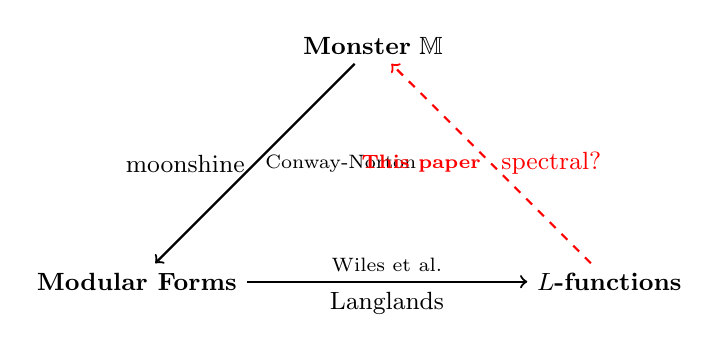
\begin{tikzpicture}[scale=2, every node/.style={font=\small}]
\node (M) at (0, 1.5) {\textbf{Monster} $\mathbb{M}$};
\node (F) at (-1.5, 0) {\textbf{Modular Forms}};
\node (L) at (1.5, 0) {\textbf{$L$-functions}};
\draw[->, thick] (M) -- node[left] {moonshine} node[right] {\scriptsize Conway-Norton} (F);
\draw[->, thick] (F) -- node[below] {Langlands} node[above] {\scriptsize Wiles et al.} (L);
\draw[->, thick, dashed, red] (L) -- node[right] {spectral?} node[left] {\scriptsize \textbf{This paper}} (M);
\end{tikzpicture}
\end{center}

The exponential sums at $j$-function coefficient scales provide supporting evidence. At the McKay scale $c_1 = 196884$, the normalized sum $|S_{100}(r_{c_1})|/N = 0.243$ is notably elevated above the $c_0 = 744$ value of 0.032, consistent with the moonshine module structure.


%% =========================================================================
\section{Discussion and Open Problems}
\label{sec:discussion}
%% =========================================================================

\subsection{What would constitute proof}

\begin{enumerate}[label=\textbf{P\arabic*.}]
\item \textbf{Scale.} Reproduce exponential sums with $10^6$+ Riemann zeros (Odlyzko tables). The current 100-zero computation has insufficient power.
\item \textbf{Character theory.} Derive the Monster prime scales $r_p = \ln p/(2\pi)$ from the character theory of $V^\natural$, not just from the primes dividing $|\mathbb{M}|$.
\item \textbf{K3 convergence.} Show that the K3 moduli optimization converges to a Ricci-flat metric as the number of zeros increases, connecting to the Yau theorem.
\item \textbf{Selberg--explicit formula bridge.} Connect the Selberg trace formula on K3 to the explicit formula for $\psi(x)$, providing a theoretical mechanism for K3-Zeta duality.
\item \textbf{E8 exponent overlap.} Prove that the 87.5\% overlap between $E_8$ exponents and Monster primes is not coincidental, e.g., via discriminant theory of sublattices.
\end{enumerate}

\subsection{Risk assessment}

This is the highest-risk conjecture in our research program. If true, it would connect three of the deepest objects in mathematics (K3 surfaces, Riemann zeros, and the Monster group). The structural evidence --- $E_8$ overlap, $\chi(K3) = 24 = \Omega$, the $j$-function coefficient anomaly --- is suggestive but not conclusive. The definitive test requires scaling to $10^6$+ zeros with proper statistical controls.


%% =========================================================================
\begin{thebibliography}{99}

\bibitem{conway1979}
J.~H.~Conway and S.~P.~Norton, \emph{Monstrous moonshine}, Bull.\ London Math.\ Soc.\ \textbf{11} (1979), 308--339.

\bibitem{borcherds1992}
R.~E.~Borcherds, \emph{Monstrous moonshine and monstrous Lie superalgebras}, Invent.\ Math.\ \textbf{109} (1992), 405--444.

\bibitem{flm1988}
I.~Frenkel, J.~Lepowsky, and A.~Meurman, \emph{Vertex Operator Algebras and the Monster}, Academic Press, 1988.

\bibitem{wiles1995}
A.~Wiles, \emph{Modular elliptic curves and Fermat's Last Theorem}, Ann.\ Math.\ \textbf{141} (1995), 443--551.

\bibitem{odlyzko1987}
A.~M.~Odlyzko, \emph{On the distribution of spacings between zeros of the zeta function}, Math.\ Comp.\ \textbf{48} (1987), 273--308.

\bibitem{yau1977}
S.-T.~Yau, \emph{Calabi's conjecture and some new results in algebraic geometry}, Proc.\ Nat.\ Acad.\ Sci.\ \textbf{74} (1977), 1798--1799.

\bibitem{novel2026}
B.~Daugherty, S.~Ward, and Ryan, \emph{Novel and speculative mathematical results: a research compendium}, working document, March 2026.

\bibitem{dsc3engine}
B.~Daugherty, \emph{Isomorphic Engine v0.15.0}, 2026. \url{https://github.com/OriginNeuralAI/DSC-3}.

\end{thebibliography}

\end{document}
